\documentclass[xcolor=table,mathserif]{beamer}
\usepackage[UTF8,heading]{ctex}
\usepackage{gbt7714}
\usepackage{amsmath,mathtools,tkz-euclide}
\usepackage{listings}
\usepackage{xcolor}
\usepackage{tikz,pgfplots,tcolorbox}
\usepackage{caption,subcaption}
\usepackage{url}
\usepackage{multicol}
\usepackage{unicode-math}
\usepackage{NUFE}

\bibliographystyle{gbt7714-numerical}

%%%%%%%%%%%%%%%%%%%%%%%%%%%%% Slides Information %%%%%%%%%%%%%%%%%%%%%%%%%%%%%%%%%%
\title[毕业设计开题报告]{NUFE Beamer Theme: 应用经济学相关问题\\——基于XX方法的研究}
\subtitle{(毕业设计开题报告)}
\author{许益友\vspace{-0.4cm}}
\institute{南京财经大学\enspace 粮食和物资学院\vspace{-0.4cm}}
\date{\today}
\titlegraphic{\includegraphics[scale=0.2]{./Pictures/校标.pdf}}

%%%%%%%%%%%%%%%%%%%%%%%%%%%%% Slides Begin Here %%%%%%%%%%%%%%%%%%%%%%%%%%%%%%%%%%
\begin{document}

\songti\rmfamily

\begin{frame}
  \titlepage
\end{frame}

\begin{frame}{目录}
    \tableofcontents
\end{frame}

\section{选题依据}
\begin{frame}{Acknowledgements}
    \begin{enumerate}
        \item 本模板基于THU Beamer Theme调整而成,如需查阅本模板的改动,可以移步\url{https://github.com/tuna/THU-Beamer-Theme},向原作者和互联网精神致敬
        \item 本模板结束页添加了邵明柱先生为我校校训创作的篆刻作品“自谦自信,务实超越”,增强了校园和艺术气息
        \item 几处较大规模的调整:
        \begin{itemize}
            \item 封面为了突出重点,调整了文档信息的字体、字号,增强布局的设计感
            \item 配色、校标调整
            \item 正文、目录、脚注、公式等字体调整
        \end{itemize}
    \end{enumerate}
\end{frame}

\begin{frame}{为什么用Beamer?}
    \begin{enumerate}
        \item 内容第一原则,不用频繁调整格式,一个模板汇报通用
        \item 格式精确,设计理念明晰而优美,对文档元素有最自由的支配权
        \item 公式排版的绝对优势
        \item 和\LaTeX{}文件交互方便
        \item 开源软件
        \item 高标准地绘制矢量图形
    \end{enumerate}
\end{frame}

\begin{frame}[allowframebreaks]{几点说明}
    \begin{enumerate}
        \item 本模板已开源至Github,地址位于\url{https://github.com/Hhhyouy/NUFE-Beamer-Theme}
        \item 中文请使用 Xe\LaTeX{} 进行编译
        \item 尽管用于演示的幻灯片应该尽可能使用非衬线字体,更有利于低分辨率投影仪的显示效果,然而在不引进新字体的情况下,黑体密集排列的效果很差。我考虑通过字体大小来弥补衬线字体的显示缺陷。\CJKunderline{我不认同幻灯片应该少字多标题的概括性设计观念},那可能是大家没有找到更简洁美观的方法引入文字,文字的重点完全可以采用{\kaishu 字体变化}、{\bfseries 粗细变化}、{\color{Light_Yellow}颜色变化}和\octagon{框线}来体现。
        \item 如上述,为了模板的通用性,我没有引进任何新字体。使用者可以通过修改NUFE.sty中的设置来调整。更好的非衬线字体例如思源黑体可以在网上下载安装。正文使用宋体还有一个好处,如果您是教师,此模板制作的课件将非常有利于学生使用iPad的显示效果。
        \item 参考文献的著录规范按照GB/T 7714-2005的要求,使用gbt7714包,默认采用顺序编码制,如果需要调整,可参照\url{https://ctan.org/pkg/gbt7714}
        \item 选择4:3的比例是为了保证与我校大部分教室的投影仪相匹配。
    \end{enumerate}
\end{frame}

\section{研究内容和目标}
\begin{frame}[fragile]{文献概览}
    Source: Abdulkadiroğlu, A., Angrist, J. and Pathak, P. (2014), The Elite Illusion: Achievement Effects at Boston and New York Exam Schools. Econometrica, 82: 137-196.

    \begin{figure}[htp]
    \centering
    \setlength{\fboxsep}{0pt}
    \foreach \x in {1,...,3} {%
      \fbox{\includegraphics[width=0.30\textwidth, page=\x]{Article/the-elite-illusion-achievement-effects-at-boston-and-new-york-ex-2014.pdf}}
    }
    \end{figure}
\end{frame}

\begin{frame}[allowframebreaks]{大段大段文字的显示效果}
天地玄黃\enspace 宇宙洪荒\enspace 日月盈昃\enspace 辰宿列張\enspace 寒來暑往\enspace 秋收冬藏\enspace 閏馀成歲\enspace 律呂調陽\enspace 雲騰致雨\enspace 露結爲霜\enspace 金生麗水\enspace 玉出昆岡\enspace 劍號巨阙\enspace 珠稱夜光\enspace 果珍李柰\enspace 菜重芥姜\enspace 海鹹河淡\enspace 鱗潛羽翔\enspace 龍師火帝\enspace 鳥官人皇\enspace 始制文字\enspace 乃服衣裳\enspace 推位讓國\enspace 有虞陶唐\enspace 吊民伐罪\enspace 周發殷湯\enspace 坐朝問道\enspace 垂拱平章\enspace 愛育黎首\enspace 臣伏戎羌\enspace 遐迩一體\enspace 率賓歸王\enspace 鳴鳳在竹\enspace 白駒食場\enspace 化被草木\enspace 賴及萬方\enspace 

蓋此身髪\enspace 四大五常\enspace 恭惟鞠養\enspace 豈敢毀傷\enspace 女慕貞潔\enspace 男效才良\enspace 知過必改\enspace 得能莫忘\enspace 罔談彼短\enspace 靡恃己長\enspace 信使可複\enspace 器欲難量\enspace 墨悲絲染\enspace 詩贊羔羊\enspace 景行維賢\enspace 克念作聖\enspace 德建名立\enspace 形端表正\enspace 空谷傳聲\enspace 虛堂習聽\enspace 禍因惡積\enspace 福緣善慶\enspace 

尺璧非寶\enspace 寸陰是競\enspace 資父事君\enspace 曰嚴與敬\enspace 孝當竭力\enspace 忠則盡命\enspace 臨深履薄\enspace 夙興溫凊\enspace 似蘭斯馨\enspace 如松之盛\enspace 川流不息\enspace 淵澄取映\enspace 容止若思\enspace 言辭安定\enspace 笃初誠美\enspace 慎終宜令\enspace 榮業所基\enspace 籍甚無竟\enspace 學優登仕\enspace 攝職從政\enspace 存以甘棠\enspace 去而益詠\enspace 樂殊貴賤\enspace 禮別尊卑\enspace 上和下睦\enspace 夫唱婦隨\enspace 外受傅訓\enspace 入奉母儀\enspace 諸姑伯叔\enspace 猶子比兒\enspace 孔懷兄弟\enspace 同氣連枝\enspace 交友投分\enspace 切磨箴規\enspace 仁慈隱恻\enspace 造次弗離\enspace 

節義廉退\enspace 顛沛匪虧\enspace 性靜情逸\enspace 心動神疲\enspace 守真志滿\enspace 逐物意移\enspace 堅持雅操\enspace 好爵自縻\enspace 都邑華夏\enspace 東西二京\enspace 背邙面洛\enspace 浮渭據泾\enspace 宮殿盤郁\enspace 樓觀飛驚\enspace 圖寫禽獸\enspace 畫彩仙靈\enspace 丙舍傍啓\enspace 甲帳對楹\enspace 肆筵設席\enspace 鼓瑟吹笙\enspace 

升階納陛\enspace 弁轉疑星\enspace 右通廣內\enspace 左達承明\enspace 既集墳典\enspace 亦聚群英\enspace 杜稿鍾隸\enspace 漆書壁經\enspace 府羅將相\enspace 路俠槐卿\enspace 戶封八縣\enspace 家給千兵\enspace 高冠陪辇\enspace 驅毂振纓\enspace 世祿侈富\enspace 車駕肥輕\enspace 策功茂實\enspace 勒碑刻銘\enspace 磻溪伊尹\enspace 佐時阿衡\enspace 奄宅曲阜\enspace 微旦孰營\enspace 桓公匡合\enspace 濟弱扶傾\enspace 绮回漢惠\enspace 說感武丁\enspace 俊乂密勿\enspace 多士寔甯\enspace 晉楚更霸\enspace 趙魏困橫\enspace 假途滅虢\enspace 踐土會盟\enspace 何遵約法\enspace 韓弊煩刑\enspace 起翦頗牧\enspace 用軍最精\enspace 宣威沙漠\enspace 馳譽丹青\enspace 九州禹迹\enspace 百郡秦並\enspace 嶽宗泰岱\enspace 禅主雲亭\enspace 雁門紫塞\enspace 雞田赤城\enspace 昆池碣石\enspace 巨野洞庭\enspace 曠遠綿邈\enspace 岩岫杳冥\enspace 治本于農\enspace 務資稼穑\enspace 俶載南畝\enspace 我藝黍稷\enspace 稅熟貢新\enspace 勸賞黜陟\enspace 孟轲敦素\enspace 史魚秉直\enspace 庶幾中庸\enspace 勞謙謹敕\enspace 聆音察理\enspace 鑒貌辨色\enspace 贻厥嘉猷\enspace 勉其祗植\enspace 省躬譏誡\enspace 寵增抗極\enspace 殆辱近恥\enspace 林臯幸即\enspace 兩疏見機\enspace 解組誰逼\enspace 索居閑處\enspace 沈默寂寥\enspace 求古尋論\enspace 散慮逍遙\enspace 

欣奏累遣\enspace 戚謝歡招\enspace 渠荷的曆\enspace 園莽抽條\enspace 

枇杷晚翠\enspace 梧桐蚤凋\enspace 陳根委翳\enspace 落葉飄搖\enspace 

遊鹍獨運\enspace 淩摩绛霄\enspace 耽讀玩市\enspace 寓目囊箱\enspace 

易輏攸畏\enspace 屬耳垣牆\enspace 具膳餐飯\enspace 適口充腸\enspace 飽饫烹宰\enspace 饑厭糟糠\enspace\enspace 親戚故舊\enspace 老少異糧\enspace 妾禦績紡\enspace 侍巾帷房\enspace 纨扇圓絜\enspace 銀燭炜煌\enspace\enspace 晝眠夕寐\enspace 藍筍象床\enspace 弦歌酒宴\enspace 接杯舉觞\enspace 矯手頓足\enspace 悅豫且康\enspace\enspace 嫡後嗣續\enspace 祭祀烝嘗\enspace 稽颡再拜\enspace 悚懼恐惶\enspace 箋牒簡要\enspace 顧答審詳\enspace\enspace 骸垢想浴\enspace 執熱願涼\enspace 驢騾犢特\enspace 駭躍超骧\enspace 誅斬賊盜\enspace 捕獲叛亡

布射僚丸\enspace 嵇琴阮嘯\enspace 恬筆倫紙\enspace 鈞巧任釣\enspace 釋紛利俗\enspace 竝皆佳妙

毛施淑姿\enspace 工颦妍笑\enspace 年矢每催\enspace 曦晖朗曜\enspace 璇玑懸斡\enspace 晦魄環照\enspace 指薪修祜\enspace 永綏吉劭\enspace 矩步引領\enspace 俯仰廊廟\enspace 束帶矜莊\enspace 徘徊瞻眺\enspace 孤陋寡聞\enspace 愚蒙等诮\enspace 謂語助者\enspace 焉哉乎也

It was the best of times, it was the worst of times, it was the age of wisdom, it was the age of foolishness, it was the epoch of belief, it was the epoch of incredulity, it was the season of Light, it was the season of Darkness, it was the spring of hope, it was the winter of despair, we had everything before us, we had nothing before us, we were all going direct to Heaven, we were all going direct the other way-in short, the period was so far like the present period, that some of its noisiest authorities insisted on its being received, for good or for evil, in the superlative degree of comparison only. 

There were a king with a large jaw and a queen with a plain face, on the throne of England; there were a king with a large jaw and a queen with a fair face, on the throne of France. In both countries it was clearer than crystal to the lords of the State preserves of loaves and fishes, that things in general were settled for ever.

It was the year of Our Lord one thousand seven hundred and seventy-five. Spiritual revelations were conceded to England at that favoured period, as at this. Mrs. Southcott had recently attained her hve-and-twentieth blessed birthday, of whom a prophetic private in the Life Guards had heralded the sublime appearance by announcing that arrangements were made for the swallowing up of London and Westminster. Even the Cock-lane ghost had been laid only a round dozen of years, after rapping out its messages, as the spirits of this very year last past (supernaturally deficient in originality) rapped out theirs. Mere messages in the earthly order of events had lately come to the English Crown and People, from a congress of British subjects in America: which, strange to relate, have proved more important to the human race than any communications yet received through any of the chickens of the Cock-lane brood.
\end{frame}

\section{研究方案设计}
\begin{frame}{公式排版和文献引用}
    消费者最优:
    \begin{gather*}
        \max\enspace U\equiv \left(\sum_{i=1}^{\infty} q_i^\rho\right) ^{\frac{1}{\rho}}\\
        \mathrm{s.t.\enspace} R=\sum_{i=1}^{\infty} p_iq_i
    \end{gather*}

    长公式排版,来自文献中的回归模型\cite{Article2014}:
    \begin{gather*}
        y_{itk}=\alpha_{tk}+\rho_kZ_{ik}k+\eta_{itk}+(1-Z_{ik})f_{0k}(r_{ik})\\
        +Z_{ik}f_{1k}(r_{ik})+\sum_{j}\delta_{jk}d_{ij}\\
        f_{jk}(r_{ik})=\pi_{jk}r_{ik}+\xi _{jk}r_{ik}^{2}+\psi_{jk}r_{ik}^{3};\quad j=0,1
    \end{gather*}
\end{frame}

\section{主要创新点}
\begin{frame}{Economic graphic}
    \begin{columns}
        \begin{column}{0.5\textwidth}
            \begin{figure}[htp]
    \centering
    \begin{tikzpicture}[scale=0.8]
        \draw[-] (0,0) -- (5,0) node[below] {$X$};
        \draw[-] (0,0) -- (0,5) node[left] {$Y$};
        \coordinate[label=below left:$O$] (O) at (0,0);
        \draw [thick,Vintage_4] (0,4) .. controls (2, 3.5) .. (4,0)
            node[
                pos = 0.6,
                sloped,
                anchor = south west
            ] (A) {};
        \draw[thick,Vintage_4] ($(A.south east) ! 2cm ! (A.south west)$)--($(A.south west) ! 3cm ! (A.south east)$);

        \coordinate (d) at ($(A.south west) ! 2cm ! 90 : (A.south east)$);
        \coordinate (d2) at ($(d) ! 1 ! 40 : (A.south west)$);        
        \coordinate (d3) at ($(d) ! 1 ! -30 : (A.south west)$);
        \foreach \point in {A.south west}
            \fill[Vintage_4,opacity=0.5] (\point) circle (2pt);
        \tkzDrawArc[thick,Vintage_4](d,d3)(d2)
    \end{tikzpicture}
    \caption{机会成本递增情况下比较优势}
    \label{compa}
\end{figure}
        \end{column}
        \begin{column}{0.5\textwidth}
            \begin{figure}[htp]
\centering
\centering
\begin{tikzpicture}
    \draw[-] (0,3) node[above] {$Y$} -- (0,0) -- (5,0) node[right] {$X$};
    \draw[domain=1:3,thick,Vintage_4] plot(\x,{2/\x});
    \draw[domain=0:4,thick,Vintage_4] plot(\x,{-0.5*\x+2});
    \draw[domain=0:1,thick,Vintage_4] plot(\x,{-2*\x+2});
    \draw[domain=1/3:3,thick,Vintage_4] plot(\x,{0.5/\x});
    \draw[domain=0:5/2,thick,Vintage_4] plot(\x,{-0.5*\x+5/4});
    \draw[domain=1/3:3,thick,Vintage_4] plot(\x,{(25/32)/\x});
    \fill[Vintage_4,opacity=0.5] (1/2,1) circle (2pt) (2,1) circle (2pt) (5/4,5/8) circle (2pt);
    \draw[Vintage_4,dashed] (1/2,0) node[below]{1}--(1/2,1);
    \draw[Vintage_4,dashed] (2,0) node[below]{2}--(2,1);
    \draw[Vintage_4,dashed] (5/4,0) node[below]{3}--(5/4,5/8);
\end{tikzpicture}
\caption{替代效应和收入效应}\label{indef}
\end{figure}
        \end{column}
    \end{columns}
\end{frame}

\begin{frame}{Economic graphic}
    \begin{figure}[htp]
    \centering
    \begin{tikzpicture}[scale=0.8]
        \draw[-] (0,0) -- (5,0) node[below] {$K$};
        \draw[-] (0,0) -- (0,5) node[left] {实物产量};
        \draw[thick,Vintage_4,-] (2,0) node[below] {$K_0$} -- (2,5) node[right,align=right] {capital supply\\ $\longrightarrow $};
        \draw[thick,Vintage_4,dashed] (0,2.5) node[left] {$R/P,MPK$} -- (2,2.5);
        \draw[thick,Vintage_4,dashed] (4,0) -- (4,5/4) (0,5/4) node[left] {$(P_K/P)(r+\delta )$} -- (4,5/4);
        \path [domain=1:5,draw,name path=lm] plot(\x,{5/(\x)}) node [right, xshift=10] {$MPK$};
        \fill [fill = Vintage_1,fill opacity=0.5] [domain = 1:2,smooth] plot (\x,{5/(\x)}) -- (0,2.5)--(0,5); 
        \fill [fill = Vintage_3,fill opacity=0.5] (0,0)--(2,0)--(2,2.5)--(0,2.5); 
        \fill [fill = Vintage_4,fill opacity=0.5] (0,0)--(4,0)--(4,5/4)--(0,5/4);
        \draw[Vintage_4,-] (1,3) -- (3,3.5) node[right] {生产企业的利润};
        \draw[Vintage_4,-] (1,2) -- (3,2.5) node[right] {租赁企业的利润};  
        \draw[Vintage_4,-] (1,0.5) -- (2,-1) node[right] {$K_0$数量资本下租赁企业的成本};                
    \end{tikzpicture}
    \caption{生产企业和租赁企业收益的差异}\label{rent_capital}
\end{figure}
\end{frame}

\begin{frame}{表格排版}
    \begin{table}[]
        \scriptsize
        \caption{回归分析表,使用stata数据集auto.dta}
        \begin{tabular}{ccccc}
        \hline
                 & \textbf{(1)} & \textbf{(2)} & \textbf{(3)} & \textbf{(4)} \\
                 & \textbf{模型1} & \textbf{模型2} & \textbf{模型3} & \textbf{模型4} \\ \hline
        headroom & 399.215      & -580.834     & -711.568     & -606.167     \\
                 & (0.3313)     & (0.2673)     & (0.1144)     & (0.1089)     \\
        trunk    &              & 292.799**    & 114.086      & 63.306       \\
                 &              & (0.0057)     & (0.3031)     & (0.4962)     \\
        weight   &              &              & 4.753***     & 5.780***     \\
                 &              &              & (0.0001)     & (0.0000)     \\
        length   &              &              & -101.709*    & -89.032*     \\
                 &              &              & (0.0184)     & (0.0141)     \\
        foreign  &              &              &              & 3526.830***  \\
                 &              &              &              & (0.0000)     \\
        \_cons   & 4970.310***  & 3875.867**   & 1.1e+04*     & 5340.190     \\
                 & (0.0002)     & (0.0032)     & (0.0138)     & (0.1825)     \\
        R2       & 0.01         & 0.11         & 0.37         & 0.57         \\
        Adj. R2  & -0.001       & 0.089        & 0.335        & 0.534        \\
        N        & 74           & 74           & 74           & 74           \\ \hline
        \end{tabular}\label{table}
    \end{table}
    
\end{frame}

\section{时间安排}

\begin{frame}{环境和引用}
    \begin{Quotation}{四書章句集注}
        \normalsize
        \octagon{論語}子曰:“富而可求也,雖執鞭之士,吾亦爲之。如不可求,從吾所好。”{\fangsong\small 好,去聲。$\bigcirc $執鞭,賤者之事。設言富若可求,則雖身爲賤役之士以求之,亦所不辭。然有命焉,非求之可得也,則安於義理而已矣,何必徒取辱哉?$\bigcirc $\CJKunderline{蘇氏}曰:“聖人未嘗有意於求富也,豈問其可不可哉?爲此語者,特以明其決不可求爾。”$\bigcirc $\CJKunderline{楊氏}曰:“君子非惡富貴而不求,以其在天,無可求之道也。}
    \end{Quotation}
    \begin{figure}[htp]
        \centering
        \includegraphics[scale=0.03]{./Pictures/kuilong.png}
    \end{figure}
\end{frame}

\begin{frame}{环境和引用}
    \begin{block}{科斯定理}
        “有必要知道损害方是否对引起的损失负责,因为没有这种权利的初始界定,就不存在权利转让和重新组合的市场交易。但是,如果定价制度的运行毫无成本,最终的结果(产值最大化)是不受法律状况影响的。”\cite{Article1960}
    \end{block}
\end{frame}

\begin{frame}[fragile]{代码块和脚注\footnote{由于listings包没有stata的代码高亮,因此选用Python}}
    \begin{columns}
    \column{.65\textwidth}
    \begin{lstlisting}[language=Python]
#数据处理
import pandas as pd 
import numpy as np

add_value = add_value[
    add_value['Accper'].dt.year 
    > 2006
    ]
add_value.fillna(
    {'Fn05602':0},
    inplace=True
    )
add_value.dropna()
    \end{lstlisting}
    \column{.3\textwidth}
    使用Python进行数据清洗,其中最常见的两个库是pandas和numpy。两者都经过底层代码的优化,numpy的广播运算相对于直接使用Python循环快很多。
    
    代码使用\CJKunderdot{\kaishu 等宽字体},如需调整可以搜索NUFE.sty。
    \end{columns}
\end{frame}

\begin{frame}[allowframebreaks]{参考文献}
\nocite{*}
\bibliography{./Article/reference}
\end{frame}

\begin{frame}
  \begin{figure}[htp]
  \centering{
  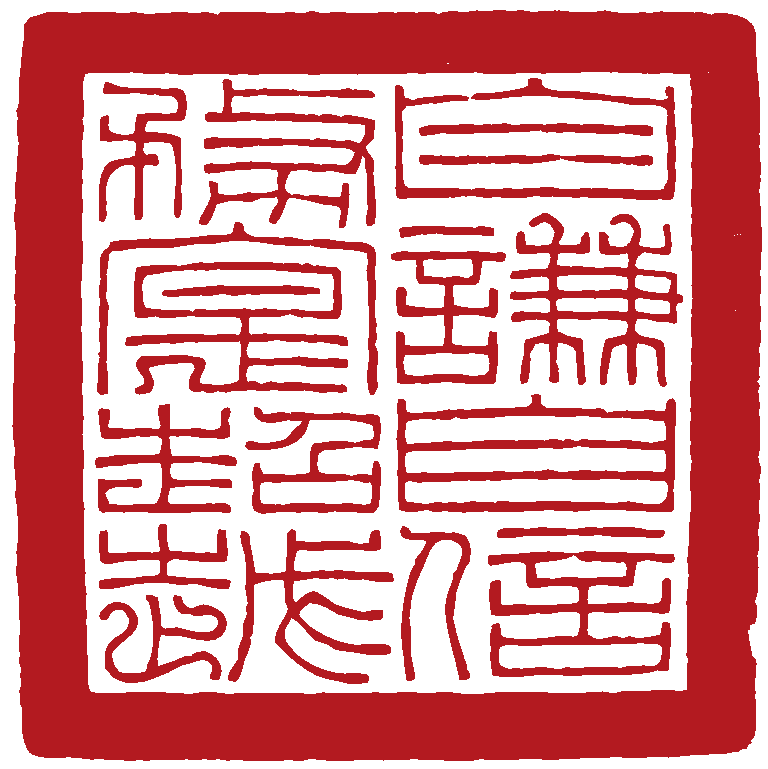
\includegraphics[scale=0.3]{./Pictures/校训篆刻.pdf}
  }
  \vspace{0.3cm}
  
  \setlength{\parindent}{0pt}
  \huge \textbf{\heiti 感谢倾听,敬请专家批评指正!}
  \end{figure}
\end{frame}

\end{document}